\documentclass[14pt,a4paper]{scrartcl}
\usepackage[utf8]{inputenc}
\usepackage[english,russian]{babel}
\usepackage{misccorr,color,ragged2e,amsfonts,amsthm,graphicx,systeme,amsmath,mdframed,lipsum}
\renewcommand\qedsymbol{$\blacksquare$}
\usepackage[normalem]{ulem}
\renewcommand*{\proofname}{\text{Доведення}}
\theoremstyle{definition}
\newtheorem{defo}{Означення}[section]
\newtheorem*{teo}{Теорема}
\newtheorem*{example}{Приклад}
\theoremstyle{remark}
\newtheorem*{remark}{Зауваження}
\theoremstyle{definition}
\newtheorem*{consequence}{Наслідок}
\theoremstyle{definition}
\newtheorem{statement}{Утверждение}[section]
\newmdtheoremenv{boxteo}{Теорема}[section]
\setlength\parindent{0pt}
\begin{document}

\def\be{\begin{equation}}
\def\ee{\end{equation}}

\def\bd{\begin{defo}}
\def\ed{\end{defo}}

\def\bbt{\begin{boxteo}}
\def\ebt{\end{boxteo}}
\textbf{10.12 3)} Побудувати скорочену ДНФ за допомогою методу Блейка:\\
$$x_1 + \overline{x_1} x_2 + \overline{x_1} \overline{x_2} x_3 + \overline{x_1}\overline{x_2}\overline{x_3}x_4 = $$
$$=x_1 + \overline{x_1}x_2 +\overline{x_1} \overline{x_2} x_3 + \overline{x_1}\overline{x_2}\overline{x_3}x_4+ x_2 + \overline{x_2} x_3 + \overline{x_2x_3}x_4 + \overline{x_1}x_3 + \overline{x_1x_3}x_4 = $$
$$= x_1 + x_2 + \overline{x_2}x_3 + \overline{x_2x_3}x_4 + \overline{x_1}x_3 + \overline{x_1x_3}x_4 =$$
$$= x_1 + x_2 + \overline{x_2}x_3 + \overline{x_2x_3}x_4 + \overline{x_1}x_3 + \overline{x_1x_3}x_4 + x_3 +\overline{x_3}x_4 + x_3 + \overline{x_3}x_4=$$
$$= x_1 + x_2  + x_3 + \overline{x_3}x_4= x_1 + x_2 + x_3 + x_4$$
\textbf{10.13 4)} Побудувати скорочену ДНФ методом Нельсона:\\
$$=
(x_1 + \overline{x_2})(x_2 + \overline{x_3}) (x_3 + \overline{x_4})(x_4 + x_1)
=$$
$$ = \begin{gathered}
  \text{ Розкриємо дужки та застосуємо поглинання }\\
  (x_1 + x_1 \overline{x_2} + x_1x_4 + \overline{x_2}x_4 )(x_2x_3 + 0 + x_2 \overline{x_4} + \overline{x_3x_4} + x_2 \overline{x_4})
\end{gathered} =
$$
$$
x_1x_2x_3 + x_1x_2 \overline{x_4} + x_1 \overline{x_3 x_4} + x_1 x_2 \overline{x_4} + 0 +0 + x_1 \overline{x_2x_3x_4} + x_1x_2x_3x_4 + 0 + 0 + 0 + 0 + 0 =
$$
$$
= x_1x_2x_3 + x_1 x_2 \overline{x_4} + x_1 \overline{x_3 x_4}
$$
\textbf{10.14 5)}
Задана функція від 3х змінних: $f(x_1, x_2, x_3) = (1110\quad 0110)$\\
Випишемо відповідні кон'юнкти$\backslash$диз'юнкти у вигляді таблиці: \\
 $$
 \left|
 \begin{gathered}
  x_1\\
  0\\
  0\\
  0\\
  0\\
  1\\
  1\\
  1\\
  1\\
 \end{gathered}
  \right|
  \left|
  \begin{gathered}
   x_2\\
   0\\
   0\\
   1\\
   1\\
   0\\
   0\\
   1\\
   1\\
  \end{gathered}
  \right|
  \left|
  \begin{gathered}
   x_3\\
   0\\
   1\\
   0\\
   1\\
   0\\
   1\\
   0\\
   1\\
  \end{gathered}
  \right|
  \left|
  \begin{gathered}
   f(x_1, x_2, x_3)\\
   1\\
   1\\
   1\\
   0\\
   0\\
   1\\
   1\\
   0\\
  \end{gathered}
  \right|
  \left|
  \begin{gathered}
   \text{кон'юнкт$\backslash$диз'юнкт}\\
 \overline{x_1} \land \overline{x_2} \land \overline{x_3}\\
 \overline{x_1} \land \overline{x_2} \land x_3\\
 \overline{x_1} \land x_2 \land \overline{x_3}\\
 x_1 \lor \overline{x_2} \lor \overline{x_3}\\
\overline{x_1} \lor x_2 \lor x_3\\
x_1\land \overline{x_2} \land x_3\\
x_1 \land x_2 \land \overline{x_3}\\
\overline{x_1} \lor \overline{x_2} \lor \overline{x_3}
  \end{gathered}
  \right|
 $$
 В результаті можемо представити задану функцію у вигляді ДДНФ, виписавши відповідні кон'юнкти:\\
 $$\textbf{ДДНФ: }  (\overline{x_1} \land \overline{x_2} \land \overline{x_3})
  \lor (\overline{x_1} \land \overline{x_2} \land x_3)
  \lor (\overline{x_1} \land x_2 \land \overline{x_3})
  \lor (x_1\land \overline{x_2} \land x_3)
  \lor (x_1 \land x_2 \land \overline{x_3})
 $$
 \pagebreak\\
 Далі, знайдемо всі тупикові ДНФ за допомогою методу карт Карно:\\
 \begin{center}
   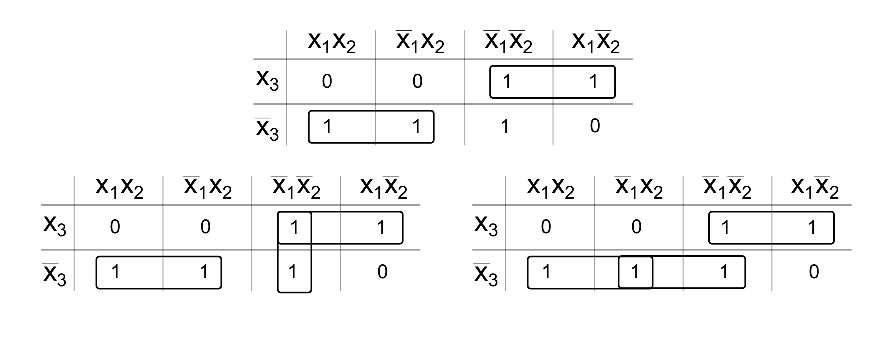
\includegraphics{karno_5.eps}
 \end{center}
 Тож, ядерні кон'юнкти: $(\overline{x_2} \land x_3)$, $(x_2 \land \overline{x_3})$.
Отримали 2 тупикові ДНФ:\\
$1.\quad (\overline{x_2} \land x_3)\lor (x_2 \land \overline{x_3}) \lor (\overline{x_1} \land \overline{x_2})$\\
$2.\quad (\overline{x_2} \land x_3)\lor (x_2 \land \overline{x_3}) \lor (\overline{x_1} \land \overline{x_3})$\\
 \\
 Знайдемо скорочену ДНФ за методом Квайна. Скористуємося спрощенною процедурою пошуку пар для застосування склеювання та поглинання. Випишемо кон'юкти ДДНФ:\\
 $$
 \begin{gathered}
1.  000\\
2.  001\\
3.  010\\
4.  101\\
5.  110\\
 \end{gathered}
\Longrightarrow
\begin{gathered}
 6. 0\text{-}0 (1,3)\\
 7. 00\text{-} (1,2)\\
 8. \text{-}01 (2,4)\\
 9. \text{-}10 (3,5)\\
\end{gathered}
\quad
\begin{gathered}
\text{За законом поглинання, викреслимо кон'юнкти 1-5.}
\end{gathered}
 $$
Далі, зведемо отримані кон'юкти у таблицю за методом Квайна - Мак-Класкі та скористаємося методом Петрика.\\
\begin{center}
\includegraphics[scale=0.5]{tabl1.png}
\end{center}
Тож, ядерні кон'юнкти: $(\overline{x_2} \land x_3)$, $(x_2 \land \overline{x_3})$.\\
\pagebreak\\
Викреслимо відповідні рядки та стовбці. Отримаємо спрощену таблицю:\\
\begin{center}
  \includegraphics[scale=0.5]{tabl2}
\end{center}
Скоротивши імпліканти, випишемо тупикові ДНФ:\\
$1.\quad (\overline{x_2} \land x_3)\lor (x_2 \land \overline{x_3}) \lor (\overline{x_1} \land \overline{x_2})$\\
$2.\quad (\overline{x_2} \land x_3)\lor (x_2 \land \overline{x_3}) \lor (\overline{x_1} \land \overline{x_3})$\\
Результат співпадає з тупиковими ДНФ, отриманими за методом карт Карно.\\
 \\
 \textbf{10.14 6)} Задана функція від 3х аргументів: $f(x_1, x_2, x_3) = (1101\quad 1011)$\\
 Випишемо відповідні кон'юнкти$\backslash$диз'юнкти у вигляді таблиці: \\
  $$
  \left|
  \begin{gathered}
   x_1\\
   0\\
   0\\
   0\\
   0\\
   1\\
   1\\
   1\\
   1\\
  \end{gathered}
   \right|
   \left|
   \begin{gathered}
    x_2\\
    0\\
    0\\
    1\\
    1\\
    0\\
    0\\
    1\\
    1\\
   \end{gathered}
   \right|
   \left|
   \begin{gathered}
    x_3\\
    0\\
    1\\
    0\\
    1\\
    0\\
    1\\
    0\\
    1\\
   \end{gathered}
   \right|
   \left|
   \begin{gathered}
    f(x_1, x_2, x_3)\\
    1\\
    1\\
    0\\
    1\\
    1\\
    0\\
    1\\
    1\\
   \end{gathered}
   \right|
   \left|
   \begin{gathered}
    \text{кон'юнкт$\backslash$диз'юнкт}\\
  \overline{x_1} \land \overline{x_2} \land \overline{x_3}\\
  \overline{x_1} \land \overline{x_2} \land x_3\\
  x_1 \lor \overline{x_2} \lor x_3\\
  \overline{x_1} \land x_2 \land x_3\\
x_1 \land \overline{x_2} \land \overline{x_3}\\
\overline{x_1} \lor x_2 \lor \overline{x_3}\\
x_1 \land x_2 \land \overline{x_3}\\
x_1 \land x_2 \land x_3
   \end{gathered}
   \right|
  $$
  В результаті можемо представити задану функцію у вигляді ДДНФ, виписавши відповідні кон'юнкти:\\
  $$\textbf{ДДНФ: }
  (\overline{x_1} \land \overline{x_2} \land \overline{x_3})\lor
  (\overline{x_1} \land \overline{x_2} \land x_3)\lor
  (\overline{x_1} \land x_2 \land x_3)\lor
(x_1 \land \overline{x_2} \land \overline{x_3})\lor
(x_1 \land x_2 \land \overline{x_3})\lor
(x_1 \land x_2 \land x_3)
  $$
  Далі, знайдемо всі тупикові ДНФ за допомогою методу карт Карно:\\
  \begin{center}
    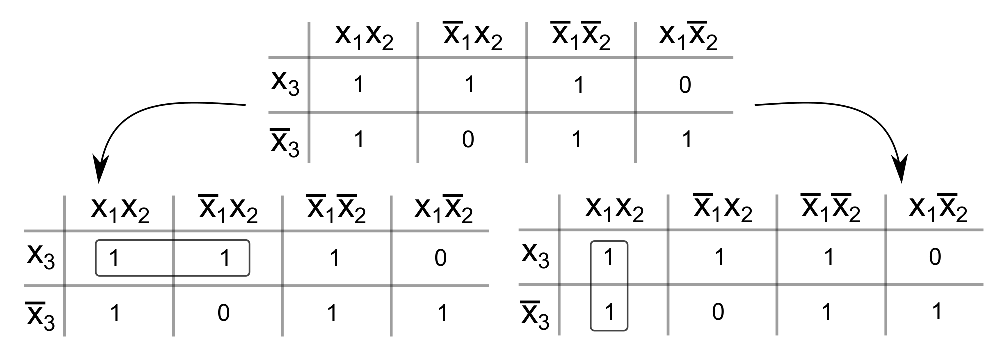
\includegraphics{karno_6.eps}
  \end{center}
  \begin{center}
    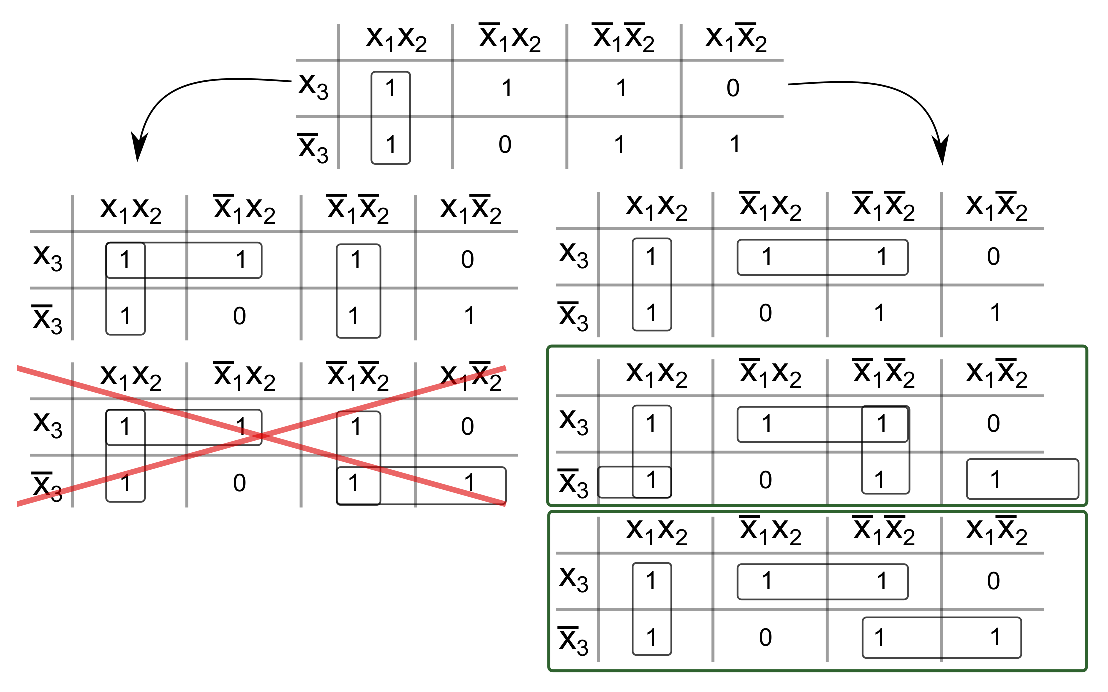
\includegraphics[scale=0.96]{karno_2.eps}
    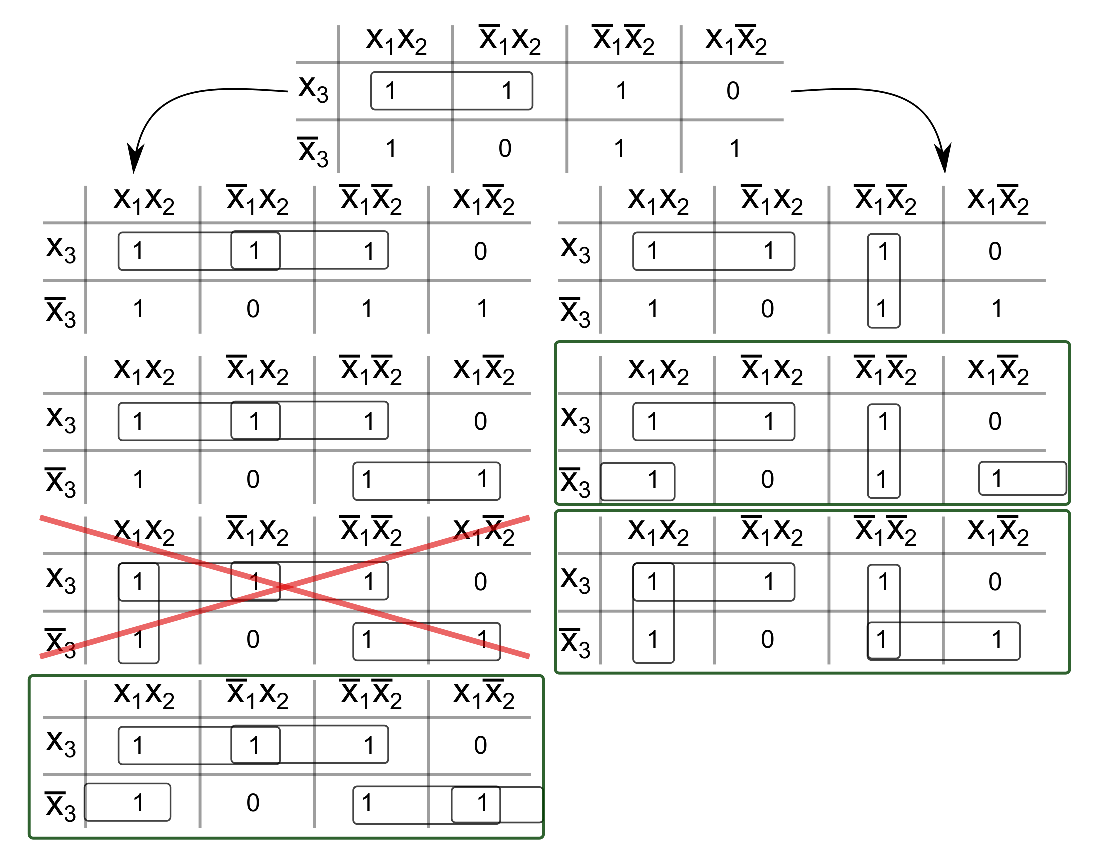
\includegraphics[scale=0.96]{karno_3.eps}
  \end{center}
Тож, ядерних імплікант немає. Отримали 5 тупикових ДНФ:\\
$T_1 = (x_1 \land x_2) \lor (x_1 \land \overline{x_3}) \lor (\overline{x_1} \land x_3) \lor (\overline{x_1} \land \overline{x_2}) $\\
$T_2 = (x_1 \land x_2) \lor (\overline{x_1} \land x_3 ) \lor (\overline{x_2}\land \overline{x_3})$\\
$T_3 = (x_2 \land x_3) \lor (x_1 \land \overline{x_3} ) \lor (\overline{x_1} \land \overline{x_2})$\\
$T_4 = (x_2 \land x_3) \lor (x_1 \land x_2 ) \lor (\overline{x_1} \land \overline{x_2}) \lor (\overline{x_2 } \land \overline{x_3})$\\
$T_5 = (x_2 \land x_3) \lor (x_1 \land \overline{ x_3}) \lor (\overline{x_1} \land x_3) \lor (\overline{x_2} \land \overline{x_3})$
 \\

  Знайдемо скорочену ДНФ за методом Квайна. Скористуємося спрощенною процедурою пошуку пар для застосування склеювання та поглинання. Випишемо кон'юкти ДДНФ:\\
  $$
  \begin{gathered}
 1.  000\\
 2.  001\\
 3.  011\\
 4.  100\\
 5.  110\\
 6.  111\\
  \end{gathered}
 \Longrightarrow
 \begin{gathered}
7. 00-(1,2)\\
8. -00(1,4)\\
9. 0-1(2,3)\\
10. -11(3,6)\\
11. 1-0(4,5)\\
12. 11-(5,6)\\
 \end{gathered}
 \quad
 \begin{gathered}
 \text{За законом поглинання, викреслимо кон'юнкти 1-6.}\\
 \text{Далі зведемо імпліканти у таблицю за методом}\\
 \text{ Квайна - Мак-Класкі та скористаємося }\\
 \text{методом Петрика.}\\
 \end{gathered}
  $$
 \begin{center}
 \includegraphics[scale=0.5]{tabl4.png}
 \end{center}
 Тож, ядерних імплікант немає. Пронумеруємо відповідні кон'юнкти. Запишемо та спростимо вираз за таблицею:\\
 \begin{center}
   \includegraphics[scale=0.5]{tabl3}
 \end{center}
 $$
(A+B)(A+C)(C+D)(B+E)(F+E)(F+D) =
 $$
 $$
=(A+BC)(С+D)(B+E)(F+ED)=
$$
$$
=(A+BC)(CB + CE + BD + DE)(F+DE)=
$$

$=(ACB + ACE + ADB + ADE + BC + BCE + BCD + BCDE)(F+ DE) =$
$
=ACEF + ADBF + ADEF + BCF + ACED + ADE + BCDE + ADBE=
$
$$
=ACEF + ADBF + BCF + ADE + BCDE
$$
 Отримали, 5 тупикових ДНФ. Скоротивши імпліканти, підставивши замість літер знайдені кон'юнкти, випишемо тупикові ДНФ:\\
 $T_1 = (x_1 \land x_2) \lor (x_1 \land \overline{x_3}) \lor (\overline{x_1} \land x_3) \lor (\overline{x_1} \land \overline{x_2}) $\\
 $T_2 = (x_1 \land x_2) \lor (\overline{x_1} \land x_3 ) \lor (\overline{x_2}\land \overline{x_3})$\\
 $T_3 = (x_2 \land x_3) \lor (x_1 \land \overline{x_3} ) \lor (\overline{x_1} \land \overline{x_2})$\\
 $T_4 = (x_2 \land x_3) \lor (x_1 \land x_2 ) \lor (\overline{x_1} \land \overline{x_2}) \lor (\overline{x_2 } \land \overline{x_3})$\\
 $T_5 = (x_2 \land x_3) \lor (x_1 \land \overline{ x_3}) \lor (\overline{x_1} \land x_3) \lor (\overline{x_2} \land \overline{x_3})$
  \\
 Результат співпадає з тупиковими ДНФ, отриманими за методом карт Карно.\\
 \\

\textbf{12.14 10)} $f(x_1, x_2, x_3, x_4) = (0001 0111 1010 1110)$\\

Відповідно, отримали такі ядерні імпліканти:
$$1. (x_1 \land \overline{x_4})  $$

$$2. (\overline{x_1} \land x_3 \land x_4)$$
Отримали прості імпліканти, тож випишемо їх, позначивши літерами, розкриємо дужки, та скористаємося законом поглиннання. Отримали вираз:
$$
(A+B)(C+D)(B+E) = (B+AE)(C+D) =
$$
$$
= BC + BD + AEC + AED
$$

Отримали 4 тупикових ДНФ:\\
$T_1 = (x_2 \land \overline{x_3} \land x_4)\lor (\overline{x_1} \land x_2 \land x_3) \lor (x_1 \land \overline{x_4}) \lor (\overline{x_1}\land x_3 \land x_4) $
\\
$T_2 = (x_1 \land \overline{x_4}) \lor (\overline{x_1}\land x_3 \land x_4) \lor (x_2 \land \overline{x_3} \land x_4) \lor (x_2 \land x_3 \land \overline{x_4}) $\\
$T_3 = (x_1 \land \overline{x_4}) \lor (\overline{x_1}\land x_3 \land x_4) \lor (\overline{x_1} \land x_2 \land x_4) \lor (x_1 \land x_2 \land \overline{x_3}) \lor (\overline{x_1} \land x_2 \land x_3)$\\
$T_4 = (x_1 \land \overline{x_4}) \lor (\overline{x_1}\land x_3 \land x_4) \lor (\overline{x_1} \land x_2 \land x_4)\lor (x_1 \land x_2 \land \overline{x_3}) \lor (x_2 \land x_3 \land \overline{x_4}) $\\
 Результат співпадає з тупиковими ДНФ, отриманими за методом карт Карно.\\

\end{document}
